\documentclass{article}

\usepackage{graphicx} % Required for the inclusion of images
\usepackage{natbib} % Required to change bibliography style to APA
\usepackage{amsmath} % Required for some math elements 


\usepackage{amssymb}
\usepackage{amsmath}
\usepackage{float}

\usepackage{caption}

\usepackage{enumitem}
\usepackage{booktabs}

\usepackage{multirow}

\usepackage{amsmath}

\usepackage{subcaption}
\captionsetup{compatibility=false}

\floatstyle{plaintop}
\restylefloat{table}

%%%%%%%%%% <GIF> %%%%%%%%%%%
\usepackage{epstopdf}

\epstopdfDeclareGraphicsRule{.gif}{png}{.png}{convert gif:#1 png:\OutputFile}
\AppendGraphicsExtensions{.gif}
%%%%%%%%%% </GIF> %%%%%%%%%%%

\setlength\parindent{0pt} % Removes all indentation from paragraphs

\renewcommand{\labelenumi}{\alph{enumi}.} % Make numbering in the enumerate environment by letter rather than number (e.g. section 6)

%\usepackage{times} % Uncomment to use the Times New Roman font

%----------------------------------------------------------------------------------------
%	DOCUMENT INFORMATION
%----------------------------------------------------------------------------------------

\title{Biometrics \\ Laboratory Report} % Title

\author{Jakub \textsc{Ciecierski}} % Author name

\date{\today} % Date for the report

\begin{document}

\maketitle % Insert the title, author and date

\begin{center}
\begin{tabular}{l r}
Date Performed: & October 30, 2015 \\ % Date the experiment was performed
\end{tabular}

\vspace{60pt}

\includegraphics[width=80mm]{res/mini.PNG} \\
\end{center}

% If you wish to include an abstract, uncomment the lines below
% \begin{abstract}
% Abstract text
% \end{abstract}

\newpage

	\tableofcontents
	
\newpage


%----------------------------------------------------------------------------------------
\section{Objective}
The objective of this study is to define an algorithm for finding a pupil in the eye image. In section~\ref{sec:method} the tools required are showcased and implemented. Further, in section~\ref{sec:pupil} the actual algorithm for extracting pupil is explained together with implementation. Results are presented in section~\ref{sec:results}. The last section is devoted to the conclusions of this study.

%----------------------------------------------------------------------------------------
\section{Methodology} 
\label{sec:method}

%----------------------------------------------------------------------------------------
%----------------------------------------------------------------------------------------
\subsection{Convolution Filters} \label{sec:conv}

The main idea of convolution filters is to modify a pixel value based on its neighbourhood.
Value of a given pixel and its neighbours are multiplied by the corresponding element in the \textit{kernel} matrix. We then sum all such products and normalize the final result. This final result is a new value for the given pixel.

Formally

\begin{center}
$I_{out}(x, y) = C_{off} + \frac{\sum_{i} \sum_{j} M(i,j) * I_{in}(x+i, y+j) }{D}$
\end{center}

where:\\
$M$ - is the kernel matrix \\
$I_{in}$ - the input image\\
$I_{out}$ - the output image\\
$C_{off}$ - offset, usually $0$ \\
$D$ - divisor, for filters equal to $\sum_i \sum_j M(i,j)$, for others just $1$\\

Kernel can be of any sizes (e.g. ($3 \times 3$), ($5 \times 5$), ($3 \times 5$), ($15 \times 15$)). The most common ones are probably ($3 \times 3$).

Notice that the summations interval of iterating the kernel matrix has been defined implicitly. To make it easier to compute corresponding pixel we fix a anchor point in the kernel matrix. The anchor point defines the origins of the kernel matrix. The figure~\ref{fig:anchor} shows an example of $3 \times 3$ kernel matrix and matrix of indices of each corresponding element. In this example, the anchor point is fixed in the middle element of kernel matrix, i.e. under value $9$.


%%%
%
% Example of Kernel Matrix
%
%%%
\begin{figure}[H]
  \centering

	\begin{tabular}{| r | r | r |}
	\hline
		$-1$ & $-1$ & $-1$ \\
	\hline
		$-1$ & $9$ & $-1$ \\
	\hline
		$-1$ & $-1$ & $-1$ \\
	\hline

	\end{tabular}

	\begin{tabular}{| r | r | r |}
	\hline
		$p_{(-1,-1)}$ & $p_{(-1,0)}$ & $p_{(-1,1)}$ \\
	\hline
		$p_{(0,-1)}$ & $p_{(0,0)}$ & $p_{(0,1)}$ \\
	\hline
		$p_{(1,-1)}$ & $p_{(1,0)}$ & $p_{(1,1)}$ \\
	\hline

	\end{tabular}
  
  {
  \caption{Kernel matrix, and their relative positions}
  \label{fig:anchor}
  }

\end{figure}



It is probably appropriate to mention that convolution filters require quite a lot of computational power. Given a kernel matrix of size $n \times m$, calculation of a single pixel require $m*n$ multiplications. Thus for big kernel matrices the computations might become very slow.

%----------------------------------------------------------------------------------------
%----------------------------------------------------------------------------------------
\subsubsection{Example}

The example in figure~\ref{fig:convo} will hopefully make it clear how exactly convolution filters define value for a given pixel. The left most matrix presents an input image, the middle one is a kernel and the right most is a final result of the current pixel. The current pixel is marked with red border. The green border however, defines the neighbourhood of that pixel. It should be clear that the anchor point is again fixed under the middle point of the kernel matrix, thus defining its origins. Further, each pixel of the image matrix is multiplied by corresponding kernel value. All products are summed. Since the only pixel that is not multiplied by $0$ has $42$, the final result is simply $42$.

%%%
%
% Example of convolution filter
%
%%%
\begin{figure}[H]
\centering

  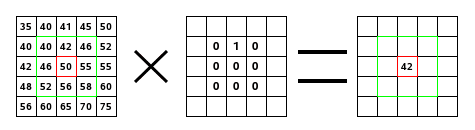
\includegraphics[width=0.9\linewidth]{res/convo.png}
  
\caption{Example of convolution filter. The computation of a new value for pixel in red border. On the left: image matrix. In the middle: kernel matrix. The right side is a new value for the current pixel}
\label{fig:convo}
\end{figure}

%----------------------------------------------------------------------------------------
%----------------------------------------------------------------------------------------
\subsubsection{Special Cases}


Finally special cases that might occur during computation of convolution filters are discussed. Firstly, however obvious, it is important that the final result is clipped to appropriate range. In case of standard RBG $[0 ,255]$, we must ensure that the final values are within this range. Finally, what happens when we compute pixels that lay at the edge of the image. For instance, for the first pixel (starting from upper left corner), the corresponding pixel of kernel matrix will simply not exist. One of the following three solutions can be applied to fix that issue.
\begin{enumerate}
	\item Compute as if there was additional row or column of pixel with values equal to the pixels at the edge.
	\item Skip the pixels with neighbours outside the edge of an image.
	\item Wrap the image. pixel outside left edge use values of pixel on the right edge.
\end{enumerate}

The method of wrapping the image has been used in the following implementations.

%----------------------------------------------------------------------------------------
%----------------------------------------------------------------------------------------
\subsubsection{Implementation}

The general algorithm flow of convolution filter is presented:
 
\begin{enumerate}
	\item For $input$ image, make a $output$ copy.
	\item For each pixel in the input image.
	\begin{enumerate}	
		\item Compute new value using kernel matrix. The neighbourhood is also taken from input image.
		\item Save new value to output image.
	\end{enumerate}
\end{enumerate}


First of all, the implementation of the main function called $compute$ is shown in figure~\ref{fig:alg_compute}. The $compute$ method calls $computeKernelColor$ for each pixel. The implementation of this method is presented in figure~\ref{fig:alg_compute_kernel}. The details of $computeKernelColor$ method are now discussed. First of all, the two loops represent the summation over the kernel matrix. The $sRange$ and $eRange$, standing for start range and end range respectively, corresponds to the indices of kernel matrix relative to the anchor point. The $getKernelPoint$ is a simply method which returns the value of kernel value for indices relative to the anchor point. This method is shown in figure~\ref{fig:alg_getKernelPoint}. Notice that $kernelMatrix$ is one-dimensional vector.


%%%
%
% 
%
%%%
\begin{figure}[H]
\centering

  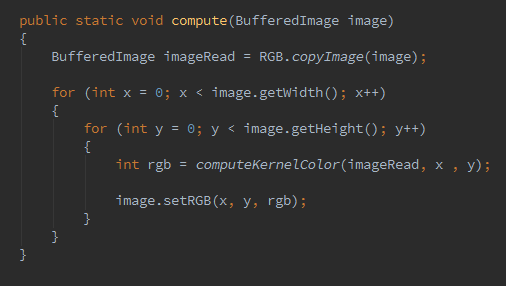
\includegraphics[width=0.9\linewidth]{res/algorithms/compute.png}
  
\caption{Main function of convolution filter}
\label{fig:alg_compute}
\end{figure}





%%%
%
% 
%
%%%
\begin{figure}[H]
\centering

  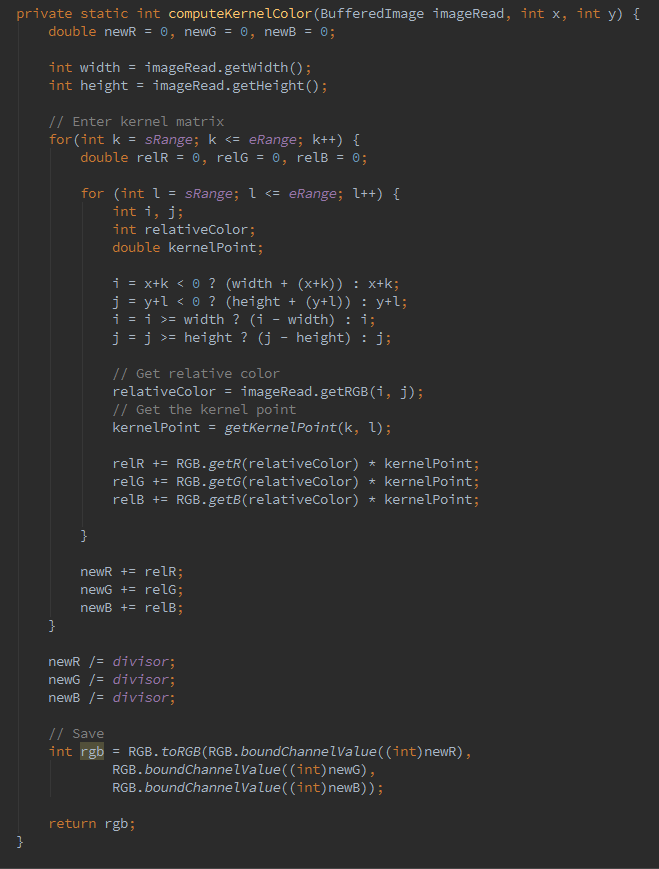
\includegraphics[width=0.9\linewidth]{res/algorithms/computeKernelColor2.png}
  
\caption{Compute Kernel}
\label{fig:alg_compute_kernel}
\end{figure}




%%%
%
% 
%
%%%
\begin{figure}[H]
\centering

  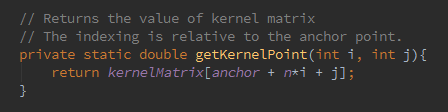
\includegraphics[width=0.9\linewidth]{res/algorithms/getKernelPoint.png}
  
\caption{Get Kernel Point}
\label{fig:alg_getKernelPoint}
\end{figure}


%----------------------------------------------------------------------------------------
%----------------------------------------------------------------------------------------
\subsection{High Pass Filter}

High pass filters underscore components of the image with high frequency. Main objective of these filters is to sharpen an image. In other words, high pass filters preserve the high frequency information and reduce low frequency information.

%%%
%
% 
%
%%%
\begin{figure}[H]
\centering

  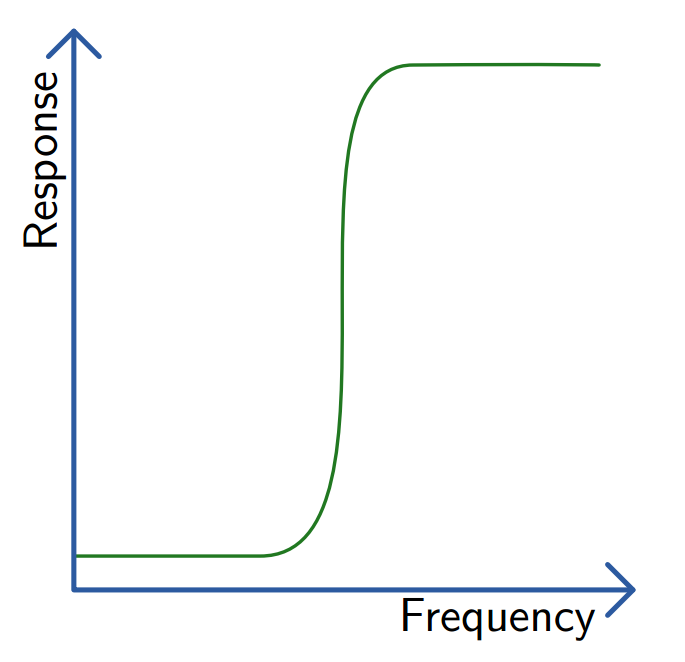
\includegraphics[width=0.5\linewidth]{res/high_pass_graph.png}
  
\caption{High Pass Filter}
\label{fig:high_pass_graph}
\end{figure}


The implementation of an example of an high pass filter called a sharpen filter is shown in figure~\ref{fig:alg_high_pass}.  The kernel is a $3 \times 3$ matrix with anchor point in the middle of that matrix. It was mentioned before that the kernel matrix is implemented using one dimensional vector. Thus it is clear to see that $kernelMatrix[anchor] = 9$. Result of applying High Pass filter is shown in figure~\ref{fig:result_high}.



%%%
%
% 
%
%%%
\begin{figure}[H]
\centering

  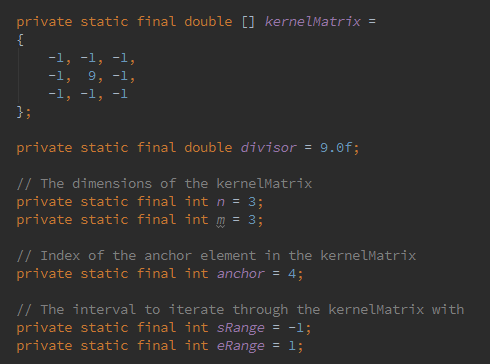
\includegraphics[width=0.9\linewidth]{res/algorithms/high_pass.png}
  
\caption{High Pass Filter}
\label{fig:alg_high_pass}
\end{figure}


%%%%
%
% Example High Pass
%
%%%%
\begin{figure}[H]
\centering

\begin{subfigure}{.5\textwidth}
  \centering
  \includegraphics[width=0.9\linewidth]{res/index.jpg}
  \caption{Original image}
  \label{fig:original_img}
\end{subfigure}%
\begin{subfigure}{.5\textwidth}
  \centering
  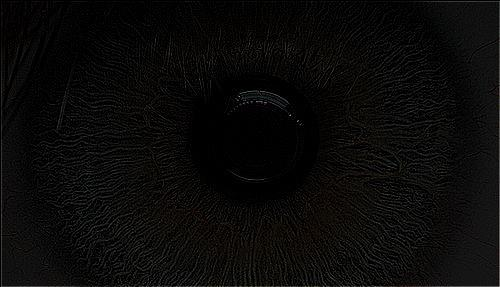
\includegraphics[width=0.9\linewidth]{res/high_pass.jpg}
  \caption{High Pass filter}
  \label{fig:gray_img}
\end{subfigure}

\caption{The original and High Pass filter}
\label{fig:result_high}
\end{figure}




%----------------------------------------------------------------------------------------
%----------------------------------------------------------------------------------------
\subsection{Low Pass Filter}

Low pass filter are used to smooth an image. By analogy, the low pass filters, preserve low frequency information and reduce the high frequency information.
Implementation presented in figure~\ref{fig:alg_low_pass}. Example of blurring an image is presented in figure~\ref{fig:result_low}.


%%%
%
% Result Low Graph
%
%%%
\begin{figure}[H]
\centering

  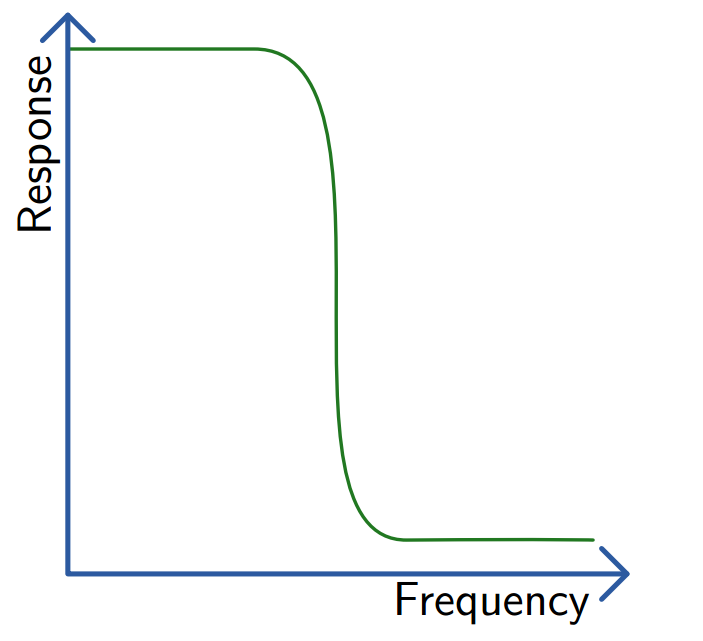
\includegraphics[width=0.5\linewidth]{res/low_pass_graph.png}
  
\caption{Low Pass Filter}
\label{fig:low_pass_graph}
\end{figure}


%%%
%
% Low Pass algoritm
%
%%%
\begin{figure}[H]
\centering

  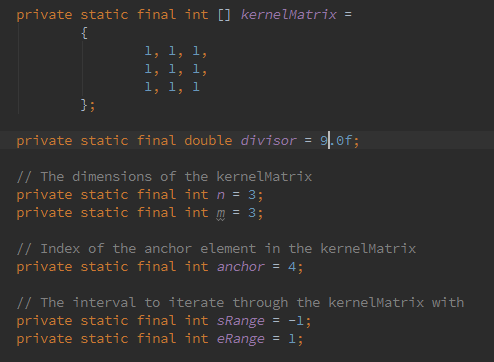
\includegraphics[width=0.9\linewidth]{res/algorithms/low_pass.png}
  
\caption{Low Pass Filter}
\label{fig:alg_low_pass}
\end{figure}





%%%
%
% Result Low Pass
%
%%%
\begin{figure}[H]
\centering

\begin{subfigure}{.5\textwidth}
  \centering
  \includegraphics[width=0.9\linewidth]{res/index.jpg}
  \caption{Original image}
  \label{fig:original_img}
\end{subfigure}%
\begin{subfigure}{.5\textwidth}
  \centering
  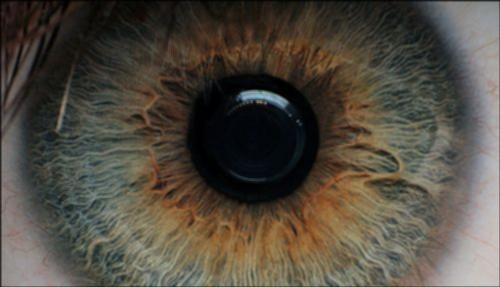
\includegraphics[width=0.9\linewidth]{res/low_pass.jpg}
  \caption{Low Pass}
  \label{fig:gray_img}
\end{subfigure}

\caption{The original and Low Pass filter}
\label{fig:result_low}
\end{figure}






%----------------------------------------------------------------------------------------
%----------------------------------------------------------------------------------------
\subsection{Gaussian Filter}
Gaussian filter is a low pass filter which is used to blur an image.
It is usually used to reduce image noise and reduce detail.

Figure~\ref{fig:alg_gauss} shows implementation.

Figure~\ref{fig:result_gauss} presents example of applyining the Gaussian filter.

%%%
%
% Gaussian Filter algorithm
%
%%%
\begin{figure}[H]
\centering

  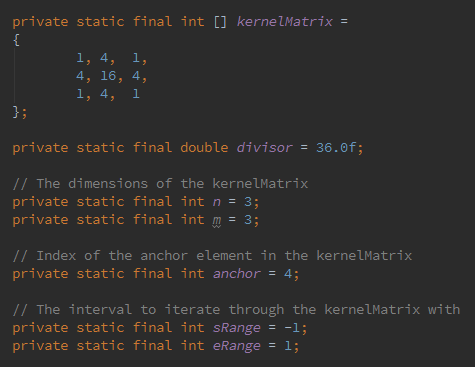
\includegraphics[width=0.9\linewidth]{res/algorithms/gaussian.png}
  
\caption{Gaussian Filter}
\label{fig:alg_gauss}
\end{figure}




%%%
%
% Gaussian Filter Result
%
%%%
\begin{figure}[H]
\centering

\begin{subfigure}{.5\textwidth}
  \centering
  \includegraphics[width=0.9\linewidth]{res/index.jpg}
  \caption{Original image}
  \label{fig:original_img}
\end{subfigure}%
\begin{subfigure}{.5\textwidth}
  \centering
  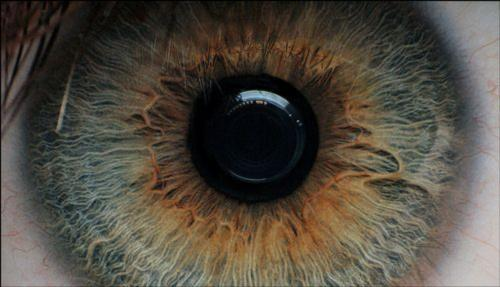
\includegraphics[width=0.9\linewidth]{res/gaussian.jpg}
  \caption{Gaussian Filter}
  \label{fig:gray_img}
\end{subfigure}

\caption{The original and gaussian filter}
\label{fig:result_gauss}
\end{figure}



%----------------------------------------------------------------------------------------
%----------------------------------------------------------------------------------------
\subsection{Sobel Filter}
The Sobel filter is used to detect edges in the image.


Calculating a new value of pixel $px$ is defined as follows:
\begin{center}
	$x = (p_2 + 2*p_3 + p_4) - (p_0 + 2*p_7 + p_6)$\\
	$y = (p_6 + 2*p_5 + p_4) - (p_0 + 2*p_1 + p_2)$\\
	$px = \sqrt[2]{x^2 + y^2}$
\end{center}

where pixels $p_0$ through $p_7$ are neighbours of $p_x$. The neighbourhood is defined in figure~\ref{fig:sobel_neigh}.

The figures~\ref{fig:compute_kernel_sobel} and~\ref{fig:compute_neigh_sobel} shows the implementation of the filter.

Finally the example of application is shown in figure~\ref{fig:result_sobel}.

%%%
%
% Sobel neighbourhood
%
%%%
\begin{figure}[H]
  \centering

	\begin{tabular}{| r | r | r |}
	\hline
		$p_0$ & $p_1$ & $p_2$ \\
	\hline
		$p_7$ & $p_x$ & $p_3$ \\
	\hline
		$p_6$ & $p_5$ & $p_4$ \\
	\hline

	\end{tabular}
  
  {
  \caption{Neighbourhood in Sobel Filter.}
  \label{fig:sobel_neigh}
  }

\end{figure}


%%%%
%
% Sobel Filter algorithm compute kernel
%
%%%%
\begin{figure}[H]
\centering

  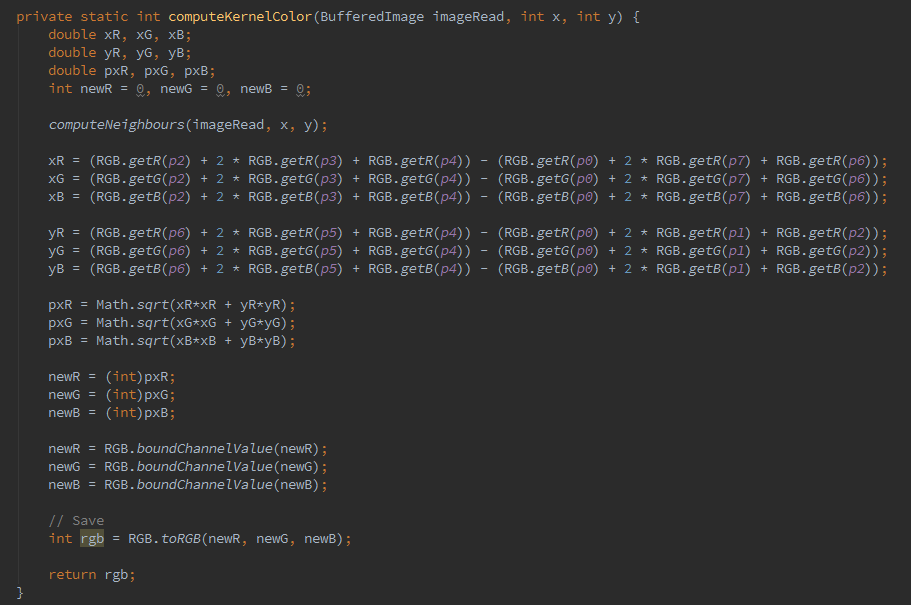
\includegraphics[width=0.9\linewidth]{res/algorithms/computeKernel_sobel.png}
  
\caption{Compute Kernel}
\label{fig:compute_kernel_sobel}
\end{figure}

%%%%
%
% Sobel Filter algorithm neighbours
%
%%%%
\begin{figure}[H]
\centering

  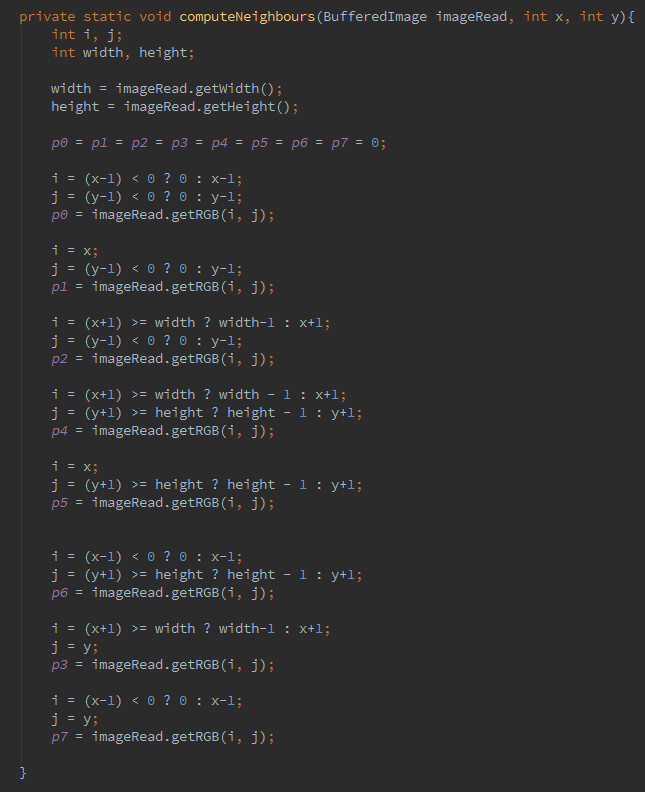
\includegraphics[width=0.9\linewidth]{res/algorithms/computeNeighbours2.png}
  
\caption{Compute Kernel}
\label{fig:compute_neigh_sobel}
\end{figure}

%%%%
%
% Sobel Filter Result
%
%%%%
\begin{figure}[H]
\centering

\begin{subfigure}{.5\textwidth}
  \centering
  \includegraphics[width=0.9\linewidth]{res/index.jpg}
  \caption{Original image}
  \label{fig:original_img}
\end{subfigure}%
\begin{subfigure}{.5\textwidth}
  \centering
  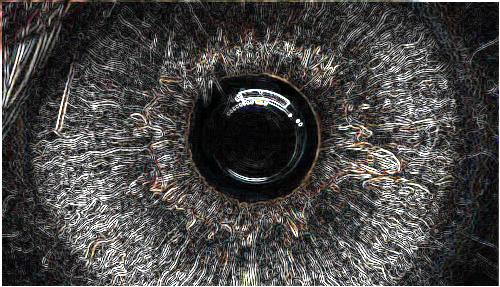
\includegraphics[width=0.9\linewidth]{res/sobel.jpg}
  \caption{Sobel filter}
  \label{fig:gray_img}
\end{subfigure}

\caption{The original and Sobel filter}
\label{fig:result_sobel}
\end{figure}




%----------------------------------------------------------------------------------------
%----------------------------------------------------------------------------------------
\subsection{Flood Fill}
\label{sec:flood}
The main objective of Flood Fill algorithm is to color all the connected pixel with the same color. Starting from a source pixel, the image will be flooded with target color as long as all the pixel remain equal to the source one.

%  \includegraphics{res/algorithms/flood.gif}

There exist different variations of Flood Fill:
\begin{enumerate}
	\item Recursive - no explicit data structure is used, only pure recursion.
 	\item Iterative
 	\begin{enumerate}
	 	\item Depth-first. Uses stack.
	 	\item Breadth-first. Uses queue.
 	\end{enumerate}
\end{enumerate}

%----------------------------------------------------------------------------------------
%----------------------------------------------------------------------------------------
\subsubsection{Implementation}

The implemented version is the Iterative Breadth-first, using the queue. The figure~\ref{fig:flood_alg} presents the method of Flood Fill. It enqueues the coordinate of the source pixel. Then, we dequeue that pixel and check whether it is equal to the background pixel. If so add four neighbours to the queue. This process is repeated until the queue is empty.


%%%%
%
% Flood Fill
%
%%%%
\begin{figure}[H]
\centering

  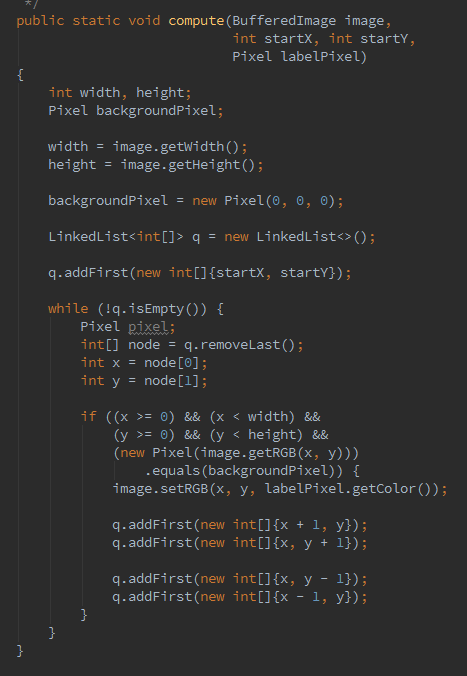
\includegraphics[width=0.9\linewidth]{res/algorithms/flood_alg.png}

\caption{The Flood Fill algorithm}
\label{fig:flood_alg}
\end{figure}


%----------------------------------------------------------------------------------------
\section{Pupil Extraction}
\label{sec:pupil}

To find the pupil on a image we must first remove as much noise as possible. To achieve this, blur filters are applied. Then, the image should be transformed to binary image - black and white. Further, Sobel filter will ensure that only edges of the pupil are left. At this point, the image should contain only one closed region - the pupil. Thus we need to apply an algorithm that finds a closed regions in an image. Once we have the interior points (points of the pupil) we can apply simple scan line algorithm to analyse the pupil. The longest line will represent diameter, and middle point of that line will be the center of the eye.
By interior of the pupil we mean all the pixels belonging to the pupil. The exterior is everything else, i.e. the background.

Formally the flow of the algorithm for original color image is as follows:

\begin{enumerate}
	\item Filter Phase - Leave only pupil's edges.
	\begin{enumerate}
			\item Apply Low Pass Filter to original image
			\item Convert image to binary image:
				\begin{enumerate}
					\item Apply Grayscale.
					\item Apply Thresholding for constant threshold.
				\end{enumerate}
			\item Apply Sobel Filter.
	\end{enumerate}
	\item Find closed region. At this point, an image should contain a black background with white edges (a circle), representing interior of the pupil.
	\begin{enumerate}
		\item Apply Flood Fill algorithm on the image starting from the upper left pixel. Label the exterior with $labelColor$ - different to black or white. All none $labelColor$ pixels represent the interior of the pupil.
		\item Fill the interior with pupil with $pupilColor$.
		\item Now, the image is binary again, with pupil's interior position known.
	\end{enumerate}
	\item Find Diameter. Apply simplified scan line algorithm
	\begin{enumerate}
		\item The longest line of the pupil will be the diameter.
		\item Center of the eye is the center of diameter line.
	\end{enumerate}
\end{enumerate}

There exist many problem with this algorithm. First of all, what blur filter to choose. Namely how much information we want to loose. Another, more obvious problem is choosing the constant for thresholding. Even though methods of estimating  threshold exist, in this experiment a constant value will be chosen by method of trail and error.

%----------------------------------------------------------------------------------------
%----------------------------------------------------------------------------------------
\subsection{Implementation}
The java implementation of the algorithm for finding the pupil is now presented. The following subsections break down the algorithm into the corresponding steps.

%----------------------------------------------------------------------------------------
%----------------------------------------------------------------------------------------
%----------------------------------------------------------------------------------------
\subsubsection{Main}


Let's start with figure~\ref{fig:pup_alg_compute} showing the parameters and the logic of the algorithm. The threshold is a constant value, in the experiment the value 4 is used. The constant $lowPassCount$ tells us how many times the image should be subjected to Low Pass filter. The $maxStartX$ and $maxEndX$ variables represent the start and end of a diameter line respectively. In analogy the $maxY$ is the y-coordinate of the diameter line. Further, the $diameter$ and $center$ are simply the length and center of the diameter line. The color to color the diameter and its center are $diameterPixel$ and $centerPixel$. Lastly, the exterior of the pupil will take color $labelPixel$ and the pupil it self will take $pupilPixel$.

The method $compute$ calls three other methods defining each step of the algorithm.

%%%%
%
% Compute
%
%%%%
\begin{figure}[H]
\centering

  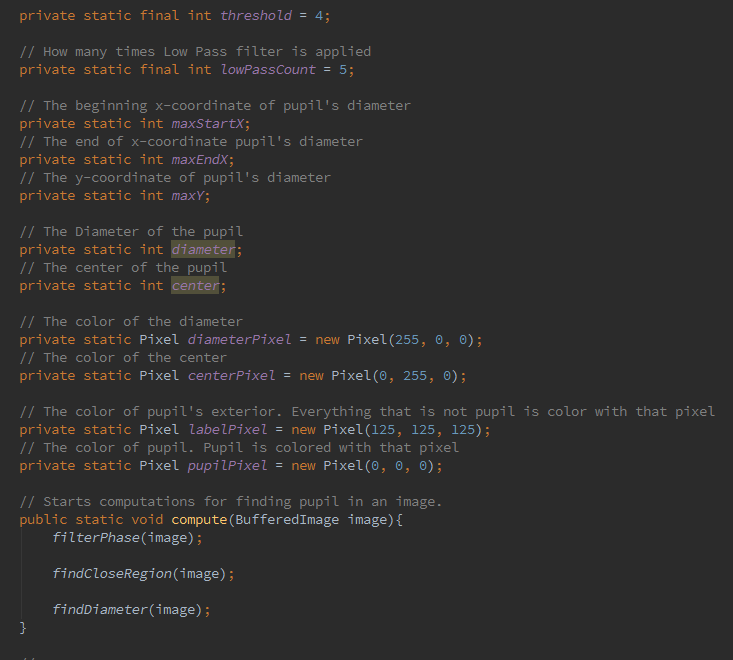
\includegraphics[width=0.9\linewidth]{res/pupil/alg/compute.png}

\caption{The parameters and compute function for pupil algorithm}
\label{fig:pup_alg_compute}
\end{figure}


%----------------------------------------------------------------------------------------
%----------------------------------------------------------------------------------------
%----------------------------------------------------------------------------------------
\subsubsection{Filter Phase}
Let's turn our attention to figure~\ref{fig:pup_alg_filter} presenting the Filter Phase. First of all, the original image is undertaken several Low Pass filters. Then the image is turned into Grayscale and the processes of blurring is repeated. Finally Theshold is computed turning the image into a binary one and Sobel filter is used to leave only the edges of the pupil.

%%%%
%
% Filter Phase
%
%%%%
\begin{figure}[H]
\centering

  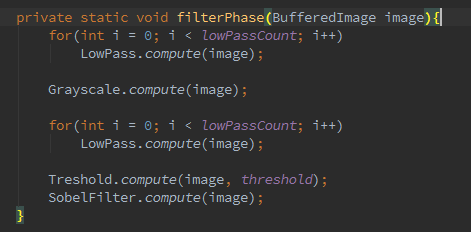
\includegraphics[width=0.9\linewidth]{res/pupil/alg/filterPhase.png}

\caption{The $filterPhase$ method}
\label{fig:pup_alg_filter}
\end{figure}

%----------------------------------------------------------------------------------------
%----------------------------------------------------------------------------------------
%----------------------------------------------------------------------------------------
\subsubsection{Find Closed Region}
At this point, we assume to have a black and white picture, where white pixel represent the edges of the pupil. Although, it is possible that the pupil it self has some white noise inside it. The process of finding the closed region of the pupil is shown in figure~\ref{fig:pup_alg_region}. Firstly, the $findClosedRegion$ methods calls Flood Fill algorithm starting from the upper left edge of the image. This process will label the exterior of the pupil with $labelPixel$. Now, we simply fill the interior of the pupil with $pupilPixel$. Notice that the interior of the pupil is simply everything that has not been filled by the Flood Fill algorithm. The $fillPupil$ method explains exactly the process of filling the pupil.

%%%%
%
% Find Closed Region
%
%%%%
\begin{figure}[H]
\centering

  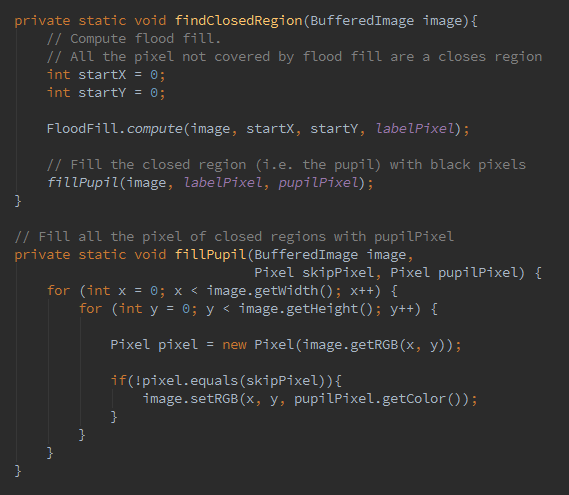
\includegraphics[width=0.9\linewidth]{res/pupil/alg/findClosedRegion.png}

\caption{The $findClosedRegion$ method}
\label{fig:pup_alg_region}
\end{figure}

%----------------------------------------------------------------------------------------
%----------------------------------------------------------------------------------------
%----------------------------------------------------------------------------------------
\subsubsection{Find Diameter}
The final phase assumes to have an binary image with no noise it in. The image should contain only the exterior and interior pixels, with regards to the pupil. The figures~\ref{fig:pup_alg_diameter} and~\ref{fig:pup_alg_scan} present the $findDiameter$ and $findLongestScanLine$ methods. Let's focus on the latter method. The $findLongestScanLine$ will iterate through every row of the image, scanning from the left to the right edge of the image. Whenever the scanline encounters a $pupilPixel$, it will fetch the next pixel and see whether it is also a $pupilPixel$. In this easy manner it will calculate a length of each horizontal line of the pupil. The longest line is chosen to be the diameter. The $findDiamter$ method after calculating the diameter will output the results and draw diameter in the binary image. The drawing methods are presented in figure~\ref{fig:pup_alg_draw}.

%%%%
%
% Find Diameter
%
%%%%
\begin{figure}[H]
\centering

  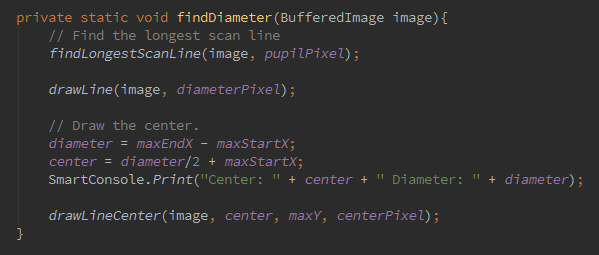
\includegraphics[width=0.9\linewidth]{res/pupil/alg/findDiameter.png}

\caption{The $findDiameter$ method}
\label{fig:pup_alg_diameter}
\end{figure}


%%%%
%
% Find Longest Scan Line
%
%%%%
\begin{figure}[H]
\centering

  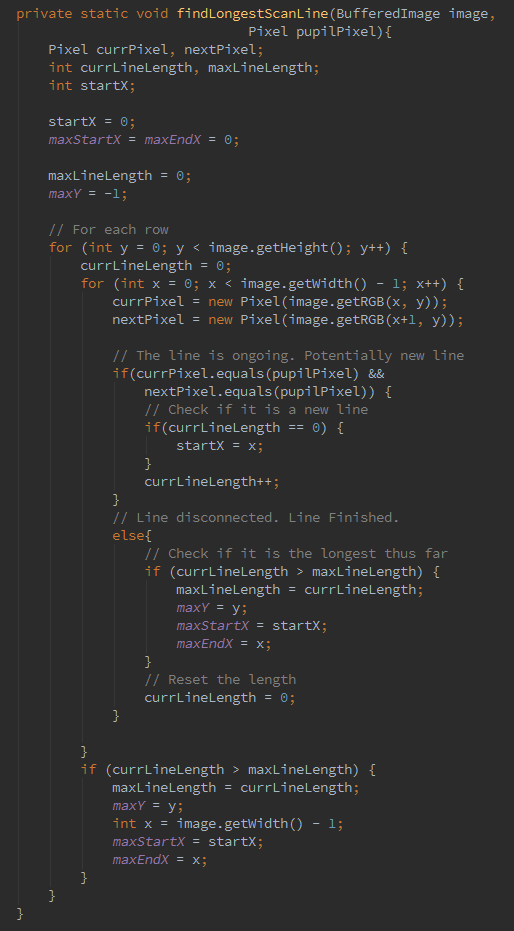
\includegraphics[width=0.9\linewidth]{res/pupil/alg/findLongestScanLine.png}

\caption{The $findLongestScanLine$ method}
\label{fig:pup_alg_scan}
\end{figure}

%%%%
%
% Draw
%
%%%%
\begin{figure}[H]
\centering

  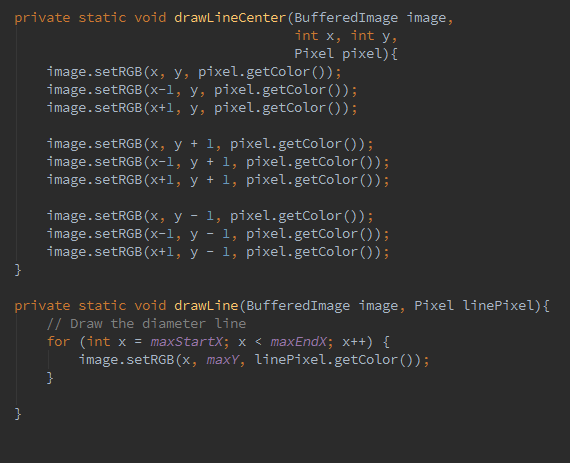
\includegraphics[width=0.9\linewidth]{res/pupil/alg/draw.png}

\caption{The methods used to draw the diameter and center}
\label{fig:pup_alg_draw}
\end{figure}


%----------------------------------------------------------------------------------------
\section{Results}
\label{sec:results}

In this section the results of the pupil extraction are presented.


%%%
%
% Originals
%
%%%
\begin{figure}[H]
\centering

\begin{subfigure}{.3\textwidth}
  \centering
  \includegraphics[width=1.0\linewidth]{res/pupil/results/index.jpg}
  \caption{Original 1}
  \label{fig:}
\end{subfigure}%
\begin{subfigure}{.3\textwidth}
  \centering
  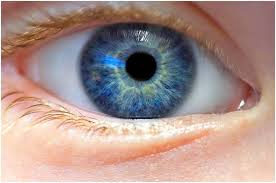
\includegraphics[width=0.9\linewidth]{res/pupil/results/eye3.jpg}
  \caption{Original 2}
  \label{fig:}
\end{subfigure}
\begin{subfigure}{.3\textwidth}
  \centering
  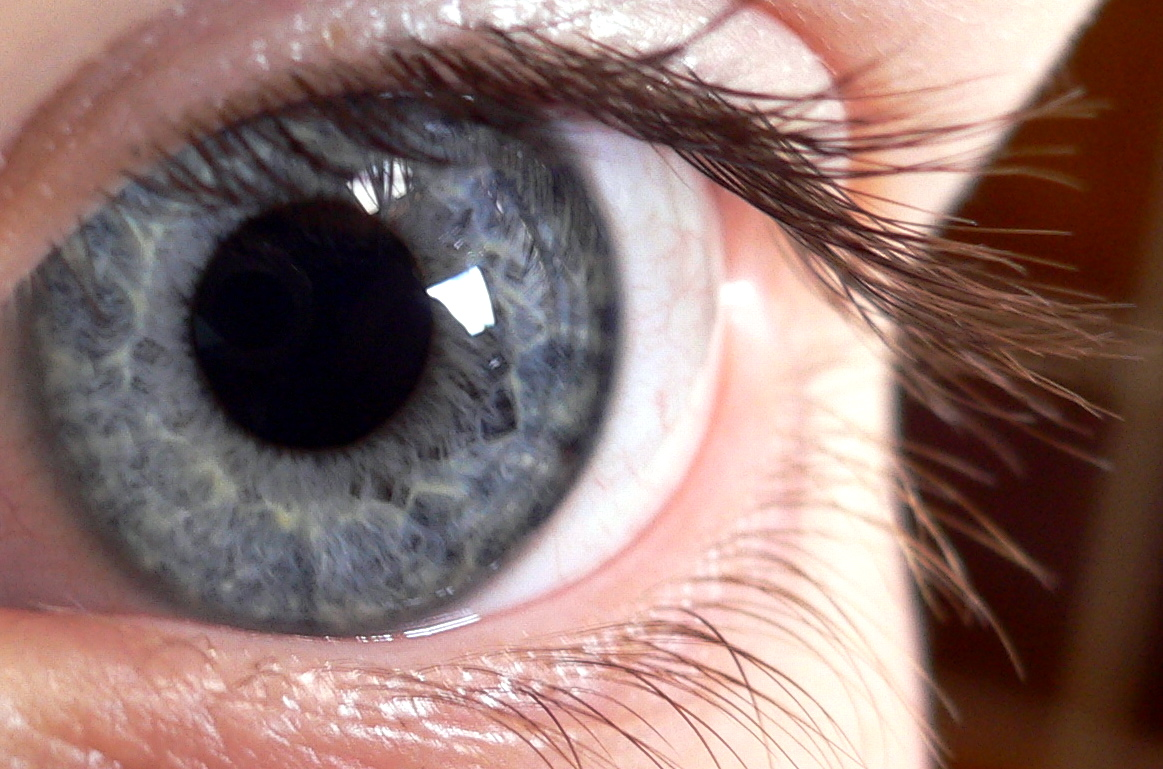
\includegraphics[width=0.9\linewidth]{res/pupil/results/eye4.jpg}
  \caption{Original 3}
  \label{fig:}
\end{subfigure}

\caption{Three images to be tested}
\label{fig:result_orgs}
\end{figure}

The figure~\ref{fig:result_orgs} shows three eye images that will be tested with previously defined algorithm. The Original 1 image will be broken down into pieces, showing effect after each step of the algorithm. The other two will have the final result presented.

The result of finding the pupil have the following structure. Each figure will present a pair of images, first one prior to transformation and the second one after. Moreover, each figure's first image will be the previous figure's second one. Hopefully the resulting effect will help to understand the process of finding the pupil interior.

The first phase of the algorithm is the filtering phase. The figure~\ref{fig:result_pup_org_low} presents the result of blurring the original image, after applying the Low Pass filter $5$ times. In figure~\ref{fig:result_pup_low_gray}, the blurred image has been subjected to Grayscale transformation. Further, in figure~\ref{fig:result_pup_gray_to_low} the Grayscale image has been blurred even more, by applying another $5$ Low Pass filters. Such image is then turned to a binary image using thresholding filter with the threshold equal to 4 - figure~\ref{fig:result_pup_gray_to_bin}. The final transformation in the first phase is the Sobel filter. The resulting image is presented in figure~\ref{fig:result_pup_bin_to_sobel}.

At this point, we constructed an image containing the edges of the pupil. The pupil it self still contains a lot noise. To clear that noise, the Flood Fill is used. The resulting effect is shown in figure~\ref{fig:result_pup_sobel_to_part_result}. The exterior of the pupil is turned into gray color, while the interior has been cleaned to the black color.

Finally the simplified scanline algorithm is applied to find the diameter. The resulting diameter and the center of the eye is shown in the figure~\ref{fig:result_pup_part_to_final}. The length of the diameter is equal to $128$ pixels.

To compare the original image with the final result, figure~\ref{fig:result_pup_org_final} has been constructed.

The result of the two other original images are presented in figures~\ref{fig:result_pup_org2_final} and~\ref{fig:result_pup_org2_final},

%%%
%
% Original to Low Pass
%
%%%
\begin{figure}[H]
\centering

\begin{subfigure}{.5\textwidth}
  \centering
  \includegraphics[width=0.9\linewidth]{res/pupil/results/index.jpg}
  \caption{Original image}
  \label{fig:}
\end{subfigure}%
\begin{subfigure}{.5\textwidth}
  \centering
  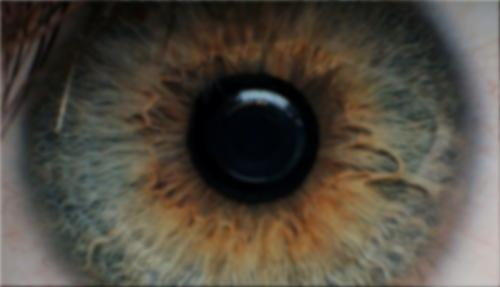
\includegraphics[width=0.9\linewidth]{res/pupil/results/org_to_low.jpg}
  \caption{Blurred image.}
  \label{fig:}
\end{subfigure}


\caption{Original to Low Pass filter}
\label{fig:result_pup_org_low}
\end{figure}


%%%
%
% Low Pass to Grayscale
%
%%%
\begin{figure}[H]
\centering

\begin{subfigure}{.5\textwidth}
  \centering
  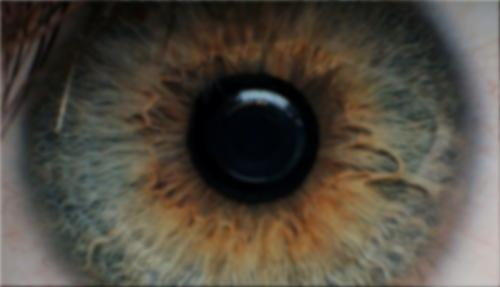
\includegraphics[width=0.9\linewidth]{res/pupil/results/org_to_low.jpg}
  \caption{Blurred image}
  \label{fig:original_img}
\end{subfigure}%
\begin{subfigure}{.5\textwidth}
  \centering
  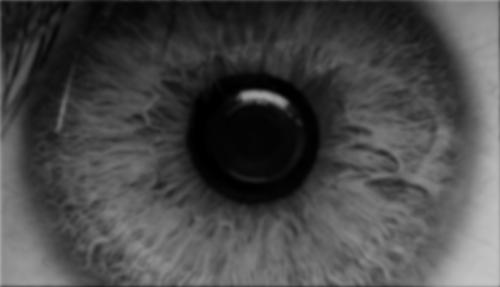
\includegraphics[width=0.9\linewidth]{res/pupil/results/low_to_gray.jpg}
  \caption{Grayscale image}
  \label{fig:gray_img}
\end{subfigure}


\caption{Low Pass to Grayscale}
\label{fig:result_pup_low_gray}
\end{figure}



%%%
%
% Grayscale to Low Pass Grayscale
%
%%%
\begin{figure}[H]
\centering

\begin{subfigure}{.5\textwidth}
  \centering
  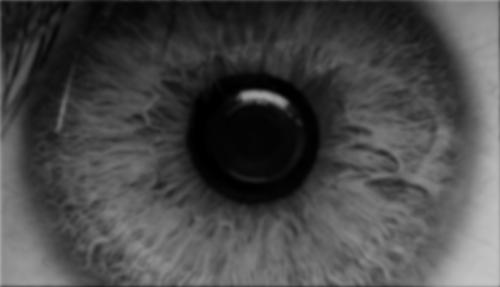
\includegraphics[width=0.9\linewidth]{res/pupil/results/low_to_gray.jpg}
  \caption{Grayscale image}
  \label{fig:original_img}
\end{subfigure}%
\begin{subfigure}{.5\textwidth}
  \centering
  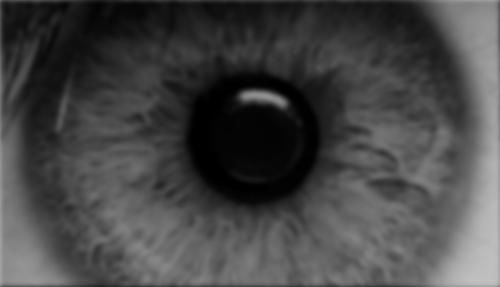
\includegraphics[width=0.9\linewidth]{res/pupil/results/gray_to_low.jpg}
  \caption{Blurred Grayscale}
  \label{fig:gray_img}
\end{subfigure}


\caption{Further blurring of the Grayscale image}
\label{fig:result_pup_gray_to_low}
\end{figure}




%%%
%
% Grayscale to Threshold
%
%%%
\begin{figure}[H]
\centering

\begin{subfigure}{.5\textwidth}
  \centering
  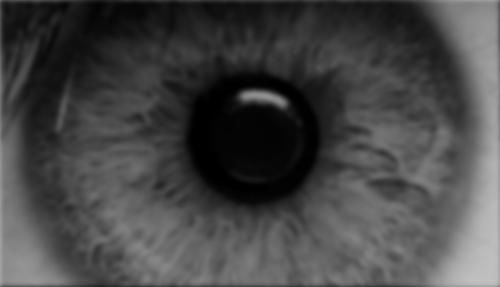
\includegraphics[width=0.9\linewidth]{res/pupil/results/gray_to_low.jpg}
  \caption{Blurred Grayscale}
  \label{fig:original_img}
\end{subfigure}%
\begin{subfigure}{.5\textwidth}
  \centering
  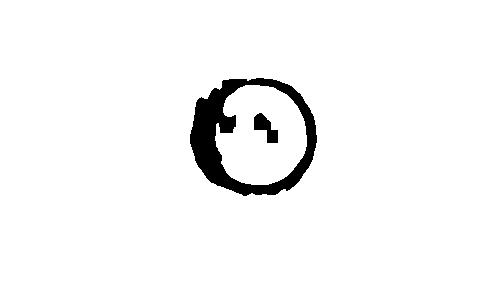
\includegraphics[width=0.9\linewidth]{res/pupil/results/lowgray_to_bin.jpg}
  \caption{Binary image}
  \label{fig:gray_img}
\end{subfigure}


\caption{Threshold fitler with value 4}
\label{fig:result_pup_gray_to_bin}
\end{figure}




%%%
%
% Threshold to Sobel
%
%%%
\begin{figure}[H]
\centering

\begin{subfigure}{.5\textwidth}
  \centering
  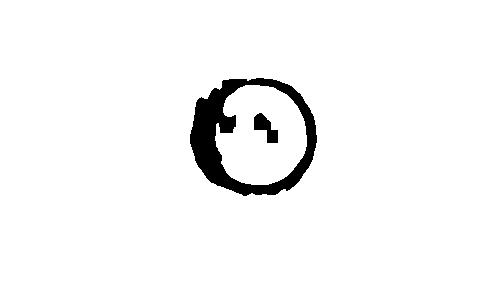
\includegraphics[width=0.9\linewidth]{res/pupil/results/lowgray_to_bin.jpg}
  \caption{Binary image}
  \label{fig:original_img}
\end{subfigure}%
\begin{subfigure}{.5\textwidth}
  \centering
  
\includegraphics[width=0.9\linewidth]{res/pupil/results/bin_to_sobel.jpg}
  \caption{Sobel filter}
  \label{fig:gray_img}
\end{subfigure}


\caption{Binary to Sobel filter}
\label{fig:result_pup_bin_to_sobel}
\end{figure}



%%%
%
% Sobel to Partial Result
%
%%%
\begin{figure}[H]
\centering

\begin{subfigure}{.5\textwidth}
  \centering
  
\includegraphics[width=0.9\linewidth]{res/pupil/results/bin_to_sobel.jpg}
  \caption{Sobel filter}
  \label{fig:original_img}
\end{subfigure}%
\begin{subfigure}{.5\textwidth}
  \centering
  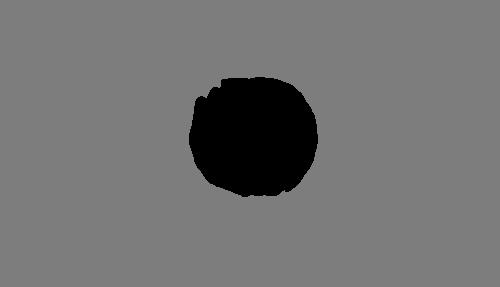
\includegraphics[width=0.9\linewidth]{res/pupil/results/sobel_to_part_result.jpg}
  \caption{The pupil}
  \label{fig:gray_img}
\end{subfigure}


\caption{The pupil is found.}
\label{fig:result_pup_sobel_to_part_result}
\end{figure}


%%%
%
% Final Result
%
%%%
\begin{figure}[H]
\centering

\begin{subfigure}{.5\textwidth}
  \centering
  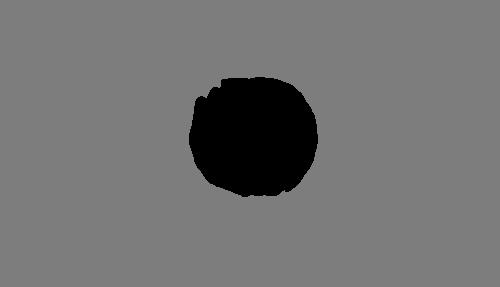
\includegraphics[width=0.9\linewidth]{res/pupil/results/sobel_to_part_result.jpg}
  \caption{The pupil}
  \label{fig:original_img}
\end{subfigure}%
\begin{subfigure}{.5\textwidth}
  \centering
  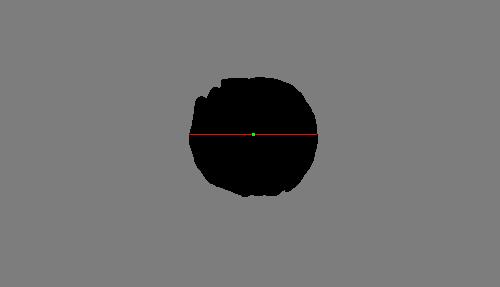
\includegraphics[width=0.9\linewidth]{res/pupil/results/part_result_to_final_result.jpg}
  \caption{The diameter and center.}
  \label{fig:gray_img}
\end{subfigure}


\caption{Drawing the diameter and center}
\label{fig:result_pup_part_to_final}
\end{figure}



%%%
%
% Original vs Final
%
%%%
\begin{figure}[H]
\centering

\begin{subfigure}{.5\textwidth}
  \centering
  \includegraphics[width=0.9\linewidth]{res/pupil/results/index.jpg}
  \caption{The original}
  \label{fig:original_img}
\end{subfigure}%
\begin{subfigure}{.5\textwidth}
  \centering
  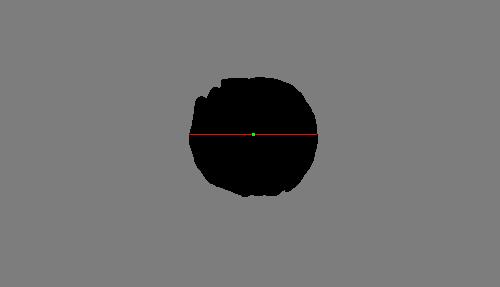
\includegraphics[width=0.9\linewidth]{res/pupil/results/part_result_to_final_result.jpg}
  \caption{The diameter and center.}
  \label{fig:gray_img}
\end{subfigure}


\caption{Original compared to Final result}
\label{fig:result_pup_org_final}
\end{figure}



%%%
%
% Original2 vs Final
%
%%%
\begin{figure}[H]
\centering

\begin{subfigure}{.5\textwidth}
  \centering
  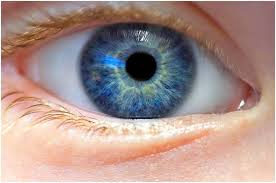
\includegraphics[width=0.9\linewidth]{res/pupil/results/eye3.jpg}
  \caption{The original 2}
  \label{fig:original_img}
\end{subfigure}%
\begin{subfigure}{.5\textwidth}
  \centering
  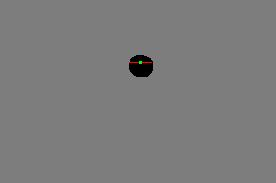
\includegraphics[width=0.9\linewidth]{res/pupil/results/eye3_pupil.jpg}
  \caption{The diameter and center.}
  \label{fig:gray_img}
\end{subfigure}


\caption{Original 2 compared to Final result. Threshold = 4. Low Pass filter application count is 4.}
\label{fig:result_pup_org2_final}
\end{figure}




%%%
%
% Original2 vs Final
%
%%%
\begin{figure}[H]
\centering

\begin{subfigure}{.5\textwidth}
  \centering
  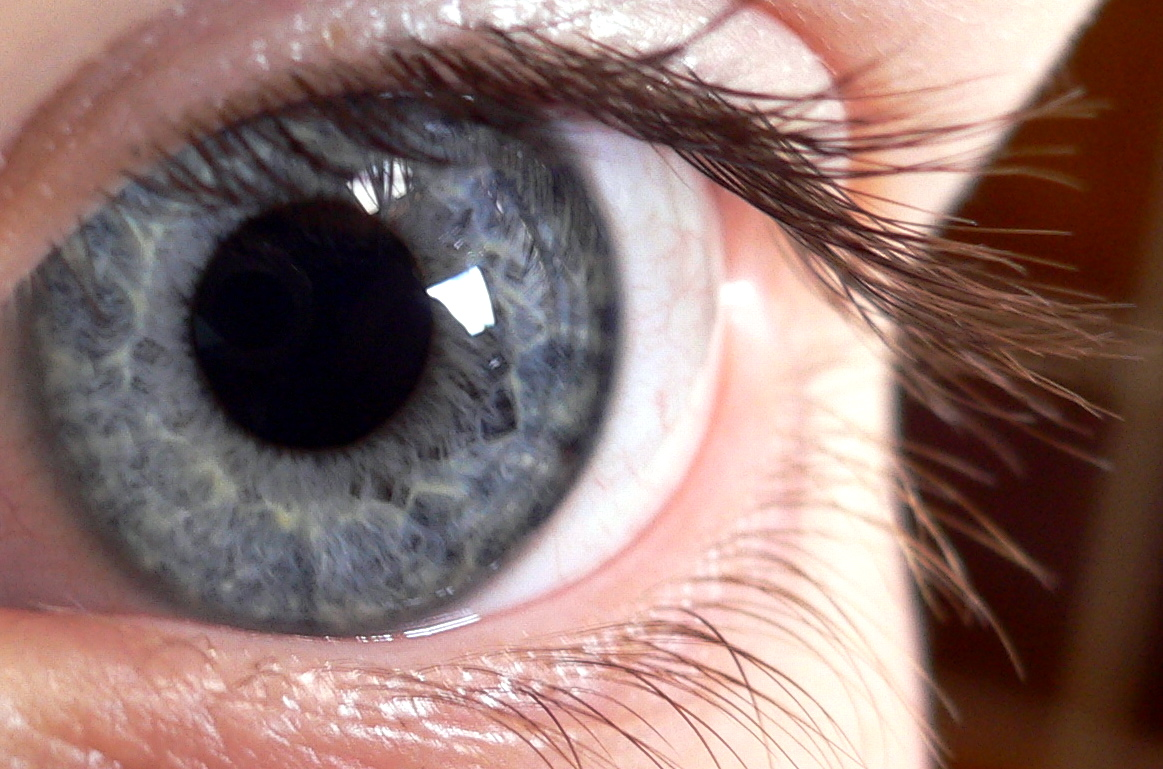
\includegraphics[width=0.9\linewidth]{res/pupil/results/eye4.jpg}
  \caption{The original 3}
  \label{fig:original_img}
\end{subfigure}%
\begin{subfigure}{.5\textwidth}
  \centering
  \includegraphics[width=0.9\linewidth]{res/pupil/results/eye4_pupil.jpg}
  \caption{The diameter and center.}
  \label{fig:gray_img}
\end{subfigure}


\caption{Original 3 compared to Final result. Threshold = 7, Low Pass filter application count is 10}
\label{fig:result_pup_org3_final}
\end{figure}




%----------------------------------------------------------------------------------------
\section{Conclusions}
\label{sec:conc}

The objective of this article focused on finding pupil in the eye image. The proper tools has been presented and finally the main algorithm for extracting pupil has been defined.

The algorithm has worked successfully for the given input image. Although the entire filtering phase has been prepared by trail and error. Further research into blurring methods and threshold evaluation is required. 

Two other randomly chosen images of the eye have been presented and the results are quite good. One of the images required change of the threshold parameter and Low Pass filter application count.


The algorithm also assumes only one closed region (pupil) in the image. The Flood Fill phase could be easily generalized using multiple region labels. One for background and others for two eyes.


%----------------------------------------------------------------------------------------
%	BIBLIOGRAPHY
%----------------------------------------------------------------------------------------

\bibliographystyle{apalike}

\bibliography{sample}
%http://docs.gimp.org/en/plug-in-convmatrix.html

%----------------------------------------------------------------------------------------


\end{document}